\documentclass{../homework}
\usepackage{ dsfont }
\usepackage{ float }

\name{Timothy Devon Morris}
\course{Me En 537}
\term{Fall 2018}
\hwnum{5}

\begin{document}
\begin{parts}[n]
    \part Problems from the Peter Corke textbook
    \begin{parts}
        \part{2-6}
        See \texttt{prob2\_6.m}. For a random $5 \times 5$ matrix it takes about 12 terms to reach precision to within $1\mathrm{e}{-4}$.
        \part{2-8}
        See \texttt{prob2\_8.m}. I got the following matrix

        \[
        \begin{bmatrix}
            0.8945 & -0.3308 & 0.3009 \\
            0.3814 & 0.9156 & -0.1274 \\
            -0.2333 & 0.2287 & 0.9451
        \end{bmatrix}
        \]
        \part{2-11}
        See \texttt{prob2\_11.m}. I chose the following matrices
        \[
            ^0R_A = 
            \begin{bmatrix}
            1 &     0    &    0      \\
            0 & \cos(\pi/3) & -\sin(\pi/3) \\
            0 & \sin(\pi/3) & \cos(\pi/3)
            \end{bmatrix}
        \]
        \[
            ^0R_B = 
            \begin{bmatrix}
            \cos(\pi/6) & -\sin(\pi/6) & 0 \\
            \sin(\pi/6) & \cos(\pi/6)  & 0 \\
            0     &    0      & 1
            \end{bmatrix}
        \]
        Thus we have that
        \[
            ^AR_B =\ ^AR_0\ ^0R_B = (\ ^0R_A)^T\ ^0R_B
            =
            \begin{bmatrix}
                0.8666 & -0.5000 & 0 \\
                -0.2500 & 0.4300 & 0.8666 \\
                -0.4333 & -0.7500 & 0.5000
            \end{bmatrix}
        \]
        and 
        \[
            ^BR_A =\ ^BR_0\ ^0R_A = (\ ^0R_B)^T\ ^0R_A
            =
            \begin{bmatrix}
                0.8666 & -0.2500 & -0.4333 \\
                -0.5000 & 0.4300 & -0.7500 \\
                0 & 0.8666 & 0.5000
            \end{bmatrix}
        \]
        For $^AR_B$ the axis-angle representation is
        \[
            \theta = 1.1589 \quad
            v = \begin{bmatrix}
            -0.8814 \\
            0.2362 \\
            0.4091
            \end{bmatrix}.
        \]
        Since we are moving in the opposite direction for $^BR_A$, the axis-angle representation is
        \[
            \theta = 1.1589 \quad
            v = \begin{bmatrix}
                0.8814 \\
                -0.2362 \\
                -0.4091
            \end{bmatrix}
        \]
        As a twist we have
        \[
            ^AS_B = 
            \begin{bmatrix}
               0 \\
               0 \\
               0 \\
               1.0223 \\
               -0.2739 \\
               -0.4744
            \end{bmatrix}
        \]
        and $^BS_A = -^AS_B$.
        \part{2-19}
        Consider the matrix product $e^Ae^B$, by terms of power series we have
        \[
            \begin{aligned}
                e^Ae^B &= \left( \sum_{i=0}^{\infty} \frac{A^i}{i!} \right) \left( \sum_{j=0}^{\infty} \frac{B^j}{j!} \right) = \sum_{i=0}^{\infty}\sum_{j=0}^{\infty} \frac{A^iB^j}{i!j!} \\
                       &\neq \sum_{i=0}^{\infty}\sum_{j=0}^{\infty} \frac{B^iA^j}{i!j!} = \left( \sum_{i=0}^{\infty} \frac{B^i}{i!} \right) \left( \sum_{j=0}^{\infty}\frac{A^j}{j!} \right) = e^Be^A
            \end{aligned}
        \]
        Because $A$ and $B$ do not necessarily commute.
        \part{3-7} See \texttt{prob3\_7.m}. Below I have plotted various trajectories that I generated using \texttt{tpoly} in matlab. The curve overshoots whenever there are velocites that are in opposite directions at the endpoints, larger in magnitude than the difference between starting and ending points, or in the opposite direction of the difference between the end points.
        \begin{figure}[H]
            \centering
            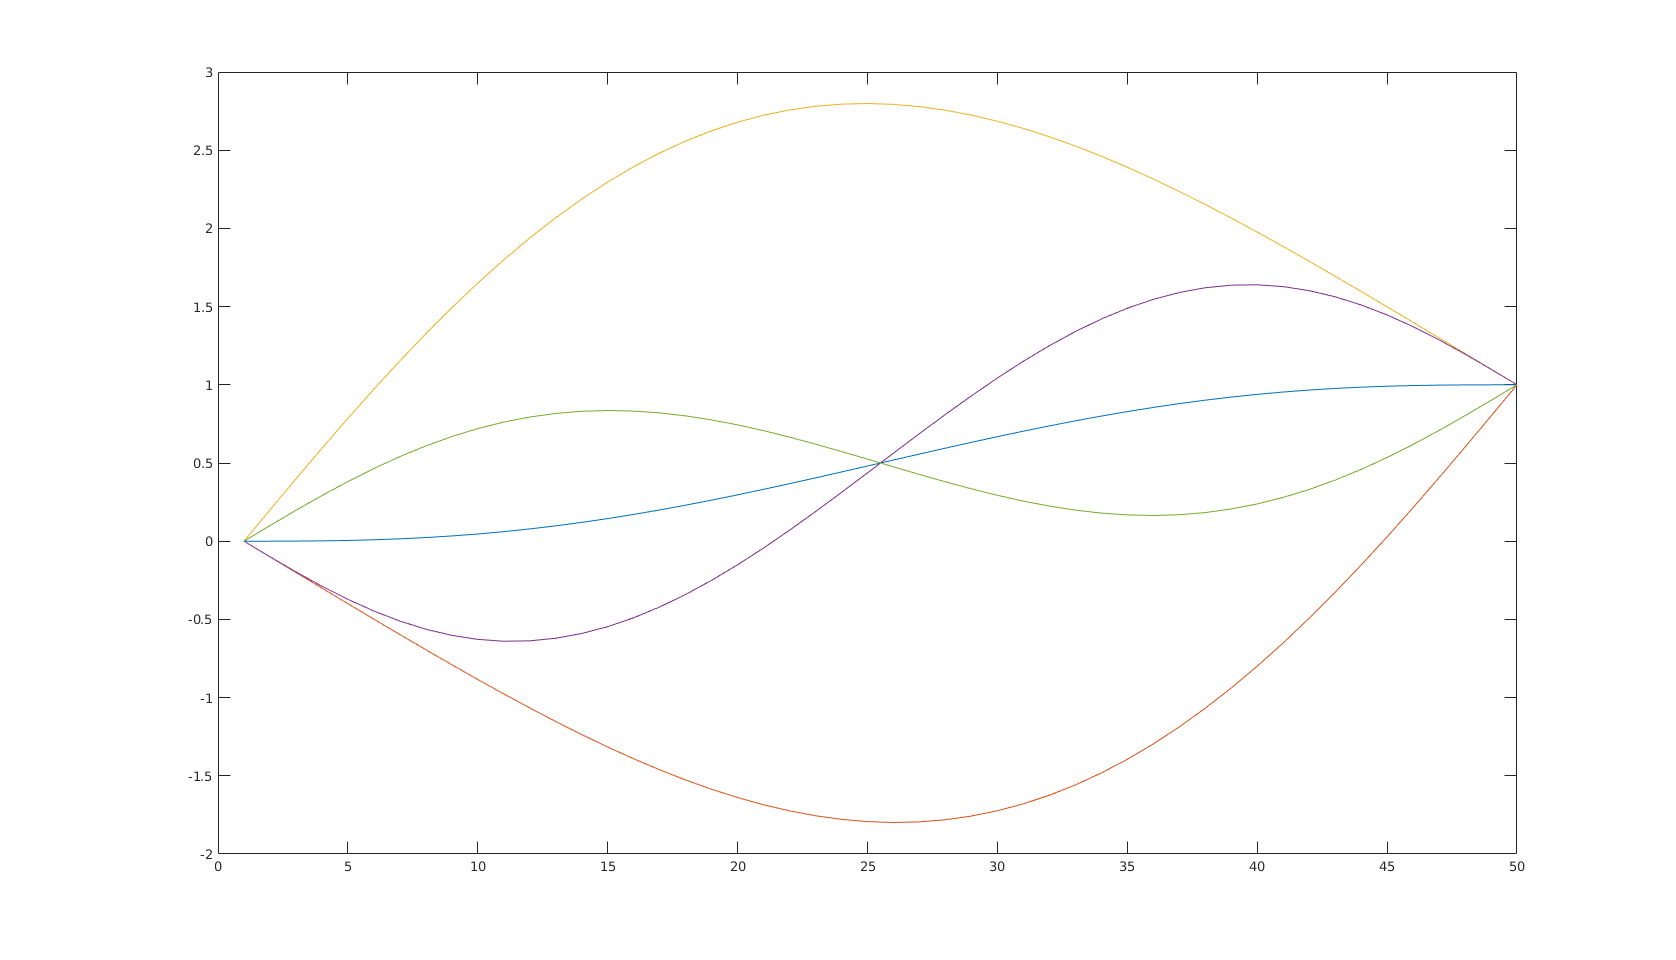
\includegraphics[scale=.3]{3_7.png}
            \label{Traj}
            \caption{Quintic Trajectories}
       \end{figure}
       \part{3-8} See \texttt{prob3\_8.m}. It seems that the smallest velocity is $0.0205$ and the largest velocity is $0.0405$. See the figure below.
       \begin{figure}[H]
            \centering
            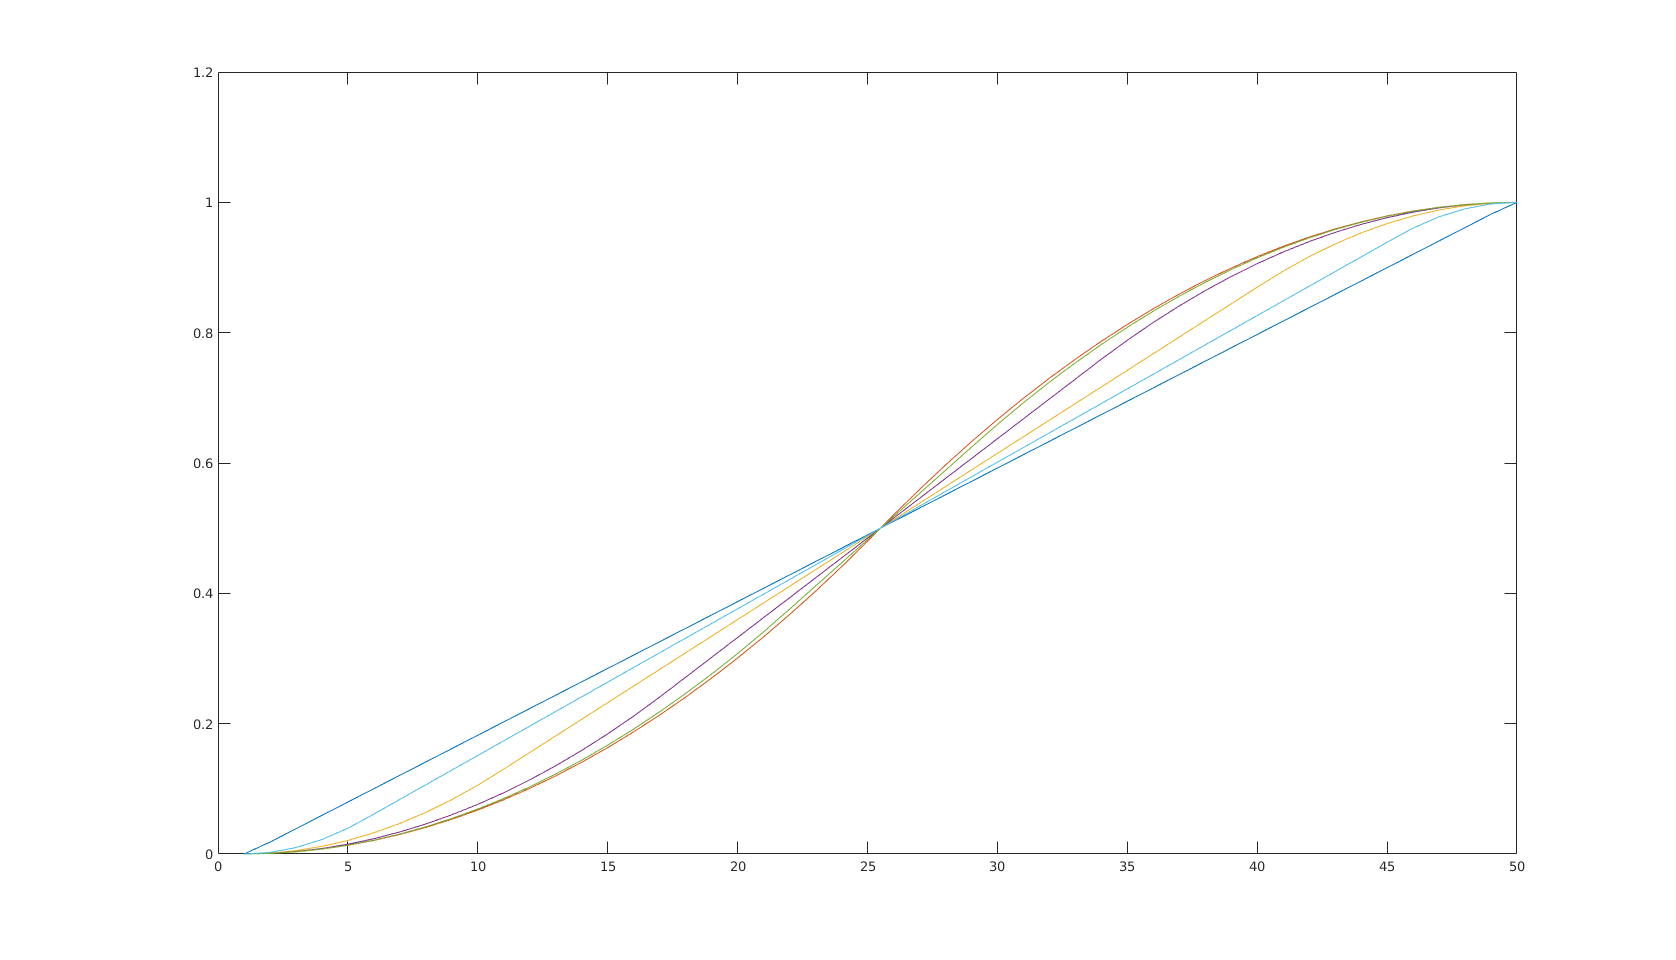
\includegraphics[scale=.3]{3_8.png}
            \label{Traj}
            \caption{Linear Segment with Parabolic Blend trajectories}
       \end{figure}
       \part{3-9} See \texttt{prob3\_9.m}. I got 77 steps for \texttt{tpoly} and 63 steps for \texttt{lspb}.

       \part{3-10} See \texttt{prob3\_10.m}. As seen in the animation, the quaternion interpolates well and is constantly moving along the same axis. The euler angles move in weird directions and kinda ``swoop'' down instead of going directly to the desired rotation.

       \part{3-13} See \texttt{prob3\_13.m}.  I commanded an initial velocity of $[10, 10]$ and final velocity of $[-5, -5]$ and got the following figure.
       \begin{figure}[H]
            \centering
            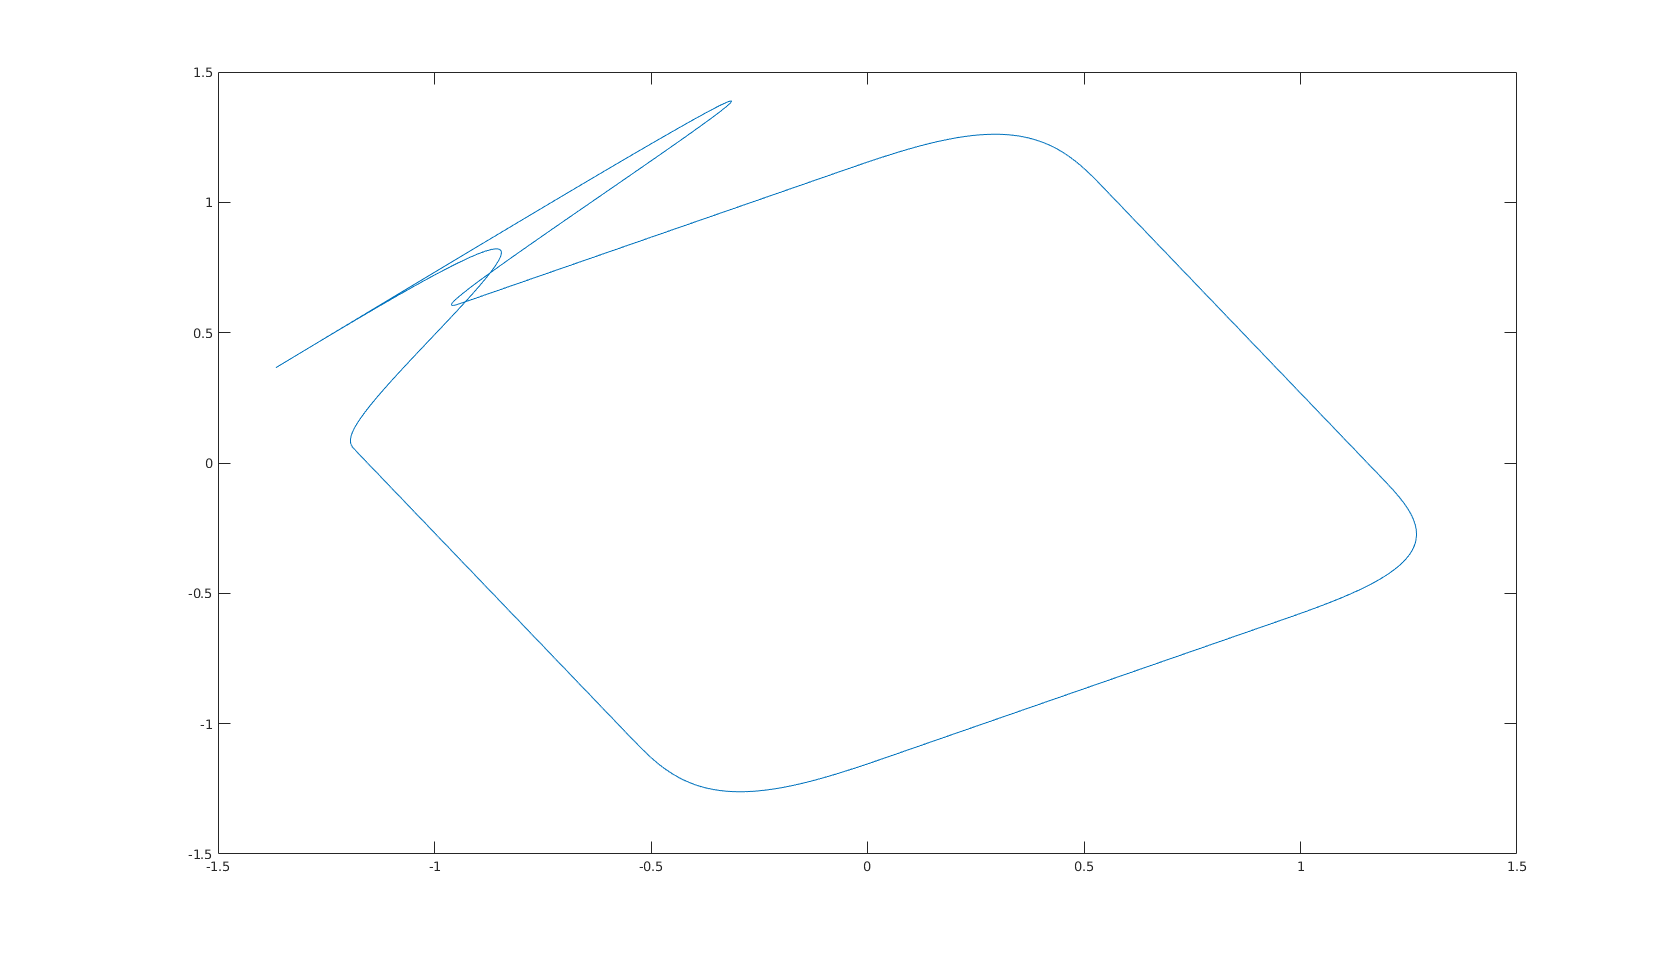
\includegraphics[scale=.3]{3_13a.png}
            \label{}
            \caption{Varying initial and final velocities}
       \end{figure}
       Obviously if you increase the acceleration time it will take more steps to complete the trajectory. The graph of how they relate is shown below.
       \begin{figure}[H]
            \centering
            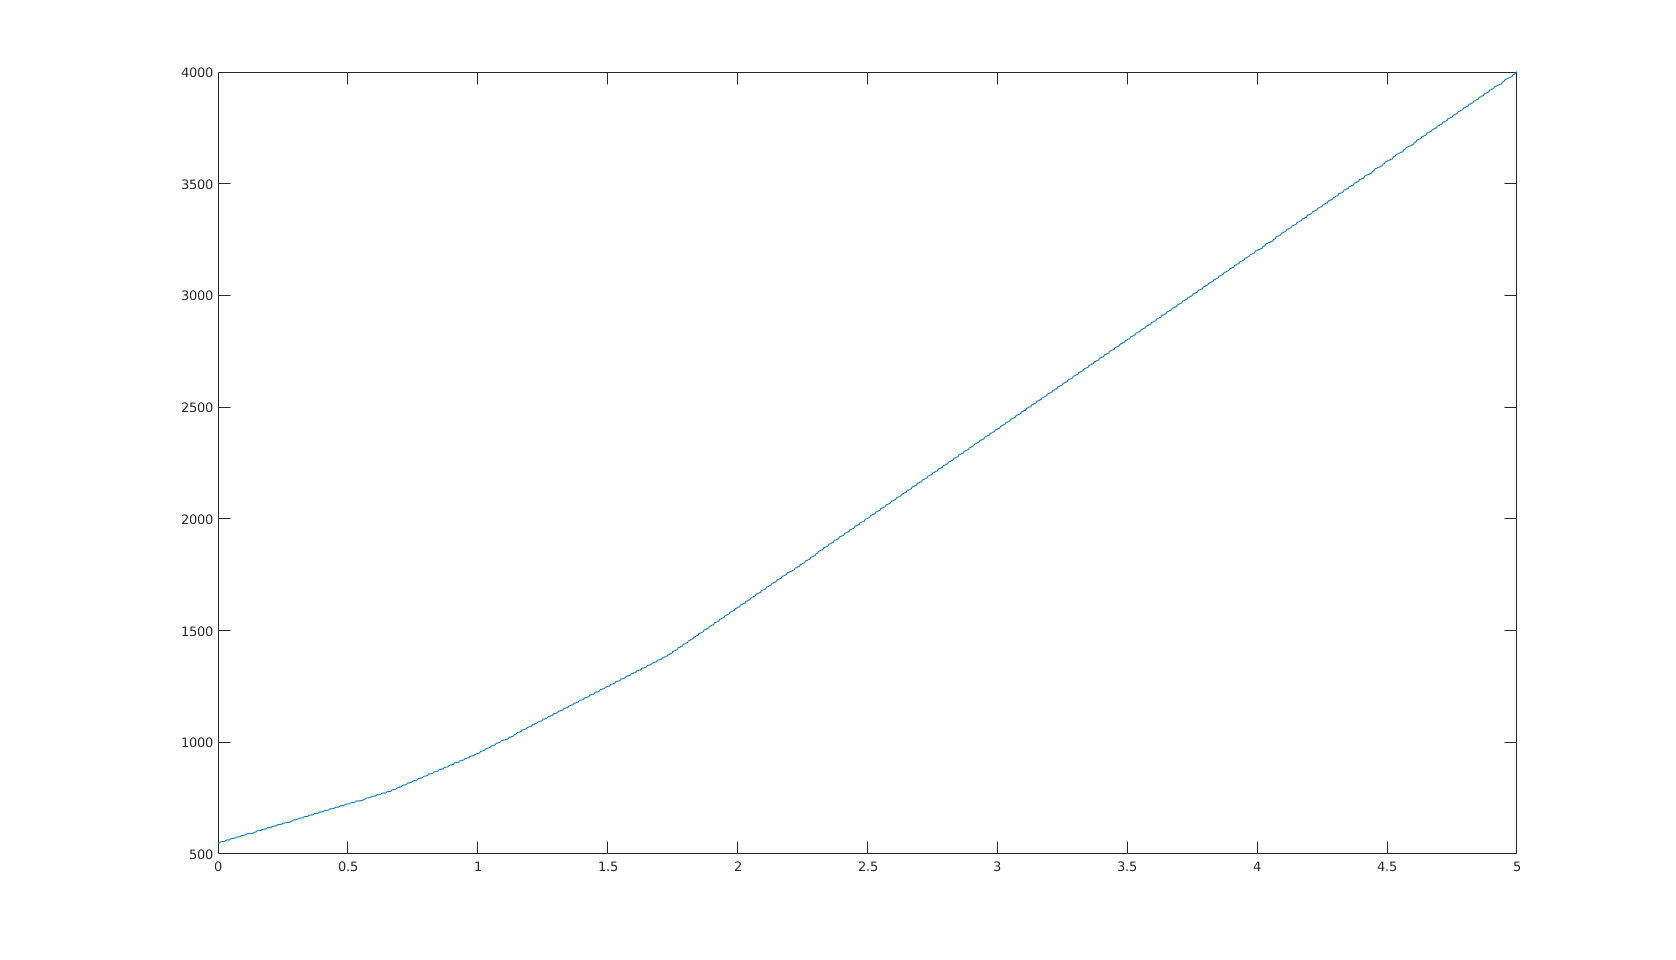
\includegraphics[scale=.3]{3_13b.png}
            \label{}
            \caption{Increasing number of steps to complete trajectory}
       \end{figure}
       \part{7-4}
    \end{parts}
    \part
    Let $\omega = [\omega_1, \omega_2, \omega_3]^T,\ p = [p_1, p_2, p_3]$, we have that
    \[
        \left[ \omega \right]_{\times} p = 
        \begin{bmatrix}
            0 & -\omega_3 & \omega_2 \\
            \omega_3 & 0 & -\omega_1 \\
            -\omega_2 & \omega_1 & 0
        \end{bmatrix}
        \begin{bmatrix}
            p_1 \\
            p_2 \\
            p_3
        \end{bmatrix}
        = 
        \begin{bmatrix}
            \omega_2p_3 - \omega_3p_2 \\
            \omega_3p_1 - \omega_1p_3 \\
            \omega_1p_2 - \omega_2p_1
        \end{bmatrix}
        =
        \omega \times p
    \]
    So the skew symmetric matrix is, in fact, consistent with the cross product.
\end{parts}
\end{document}
